\documentclass[../main.tex]{subfile}
\graphicspath{{\subfix{../images}}}
\begin{document}

在本节中,我们首先以每像素预测的方式重新制定目标检测。 接下来,我们将展示我们如何利用多级预测来提高召回率并解决重叠边界框导致的歧义。 最后,我们展示了我们提出的“centerness”分支,它有助于抑制检测到的低质量边界框并大幅提高整体性能。

\subsection{全卷积单阶段物体检测器}

令$ F_i \in \mathbbm{R}^{H\times W\times C} $是主干 CNN 第$ i $层的特征图,$s $是到该层的总步长。输入图像的ground-truth边界框定义为$\left\{ B_i \right\}$,其中 $ B_i = \left( x_0^{\left(i\right)},y_0^{\left(i\right)},x_1^{\left(i\right)},y_1^{\left(i\right)},c^{\left(i\right)} \right) \in \mathbbm{R}^4 \times \left\{ 1, 2, \ldots, C \right\}$。这里 $\left( x_0^{\left(i\right)},y_0^{\left(i\right)} \right)$和$\left( x_1^{\left(i\right)},y_1^{\left(i\right)} \right)$表示边界框的左上角和右下角的坐标。 $c^{\left(i\right)}$ 是边界框中的对象所属的类。$ C $是类的数量,对于 MS-COCO 数据集是 80。

对于特征图$ F_i $上的每个位置$\left(x, y\right)$,我们可以将其映射回输入图像的$\left( \lfloor \frac{s}{2} \rfloor + xs,  \lfloor \frac{s}{2} \rfloor + ys\right)$,它靠近位置的感受野中心$\left(x, y\right)$。与基于锚点的检测器不同,它们将输入图像上的位置视为(多个)锚框的中心,并以这些锚框为参考回归目标边界框,我们直接在该位置回归目标边界框。换句话说,我们的检测器直接将位置视为训练样本,而不是基于锚的检测器中的锚框,这与用于语义分割的 FCN 相同\cite{fcn}。

具体来说,如果位置$\left(x, y\right)$落入任何ground-truth框,则将其视为正样本,并且该位置的类标签$ c^\ast $是ground-truth框的类标签。否则它是一个负样本并且 $ c^\ast $(背景类)。除了分类标签之外,我们还有一个 4D 实向量 $\mathbf{t}^\ast = (l^\ast, t^\ast, r^\ast, b^\ast)$ 作为该位置的回归目标。这里$l^\ast, t^\ast, r^\ast$和$b^\ast$是该位置到边界框四个边的距离,如图 \ref{fig:fig1}(左)所示。如果一个位置落入多个边界框,它被认为是一个\textit{有歧义的样本}。我们简单地选择面积最小的边界框作为其回归目标。在下一节中,我们将展示通过多级预测,可以显着减少模糊样本的数量,因此它们几乎不会影响检测性能。形式上,如果位置$\left(x, y\right)$与边界框$ B_i $相关联,则该位置的训练回归目标可以表示为,
\begin{equation}\label{equ:position}
    \begin{aligned}
         & l^\ast & = & x - x_0^{\left(i\right)},  \\
         & t^\ast & = & y - y_0^{\left(i\right)},  \\
         & r^\ast & = & x_1^{\left(i\right)} - x , \\
         & b^\ast & = & y_1^{\left(i\right)} - y.
    \end{aligned}
\end{equation}
\textit{值得注意的是,FCOS 可以利用尽可能多的前景样本来训练回归器。} 它与基于锚的检测器不同,后者只将与ground-truth框具有足够高IOU的锚框作为正样本。 我们认为这可能是 FCOS 优于其基于锚的同行的原因之一。

\paragraph{网络输出。}

对应于训练目标,我们网络的最后一层预测分类标签的80D向量 $\mathbf{p}$ 和4D 向量 $\mathbf{t} = \left(l, t, r, b\right)$ 边界框坐标。 按照\cite{retinanet},我们训练$ C $个二元分类器,而不是训练多类分类器。 与\cite{retinanet}类似,我们在主干网络的特征图之后添加了四个卷积层,分别用于分类和回归分支。 此外,由于回归目标始终为正,因此我们在回归分支顶部使用$ \exp\left(x\right) $来将任何实数映射到$\left(0, \infty \right)$。 值得注意的是,FCOS 的网络输出变量比流行的每个位置有 9 个锚框的检测器\cite{retinanet, fasterrcnn}少 9 倍,。

\paragraph{损失函数。}

我们如下定义我们的训练损失函数:
\begin{equation} \label{equ:total_loss}
    \begin{aligned}
         & L\left(\left\{\mathbf{p}_{x,y}\right\},\left\{\mathbf{t}_{x,y}\right\}\right) & = & \frac{1}{N_\text{pos}}\sum_{x,y}L_\text{cls}\left( \mathbf{p}_{x,y}, c_{x,y}^\ast \right)                                                               \\
         &                                                                               & + & \frac{\lambda}{N_\text{pos}} \sum_{x, y}\mathbbm{1}_{\left\{c_{x,y}^\ast > 0\right\}}L_\text{reg}\left( \mathbf{t}_{x,y}, \mathbf{t}_{x,y}^\ast \right)
    \end{aligned}
\end{equation}
其中 $L_\text{cls}$ 是 \cite{retinanet}中的焦点损失,$L_\text{reg}$ 是 UnitBox\cite{unitbox}中的 IOU 损失。 $N_\text{pos}$ 表示正样本的数量,$\lambda$是$L_\text{reg} $的平衡权重,在本文中设置为1。求和是在特征图$ F_i $上的所有位置上计算的。 $\mathbbm{1}_{\left\{c_{x,y}^\ast > 0\right\}}$是指示函数,如果$ c^\ast_i > 0 $则为 1,否则为 0。

\paragraph{推理。}

FCOS 的推理很简单。 给定输入图像,我们通过网络将其转发并获得特征图$ F_i $上每个位置的分类分数$\mathbf{p}_{x,y}$和回归预测$\mathbf{t}_{x,y}$。按照\cite{retinanet},我们选择$p_{x,y} > 0.05 $的位置作为正样本并反转方程\ref{equ:position}获得预测的边界框。

\subsection{为FCOS使用FPN进行多层级预测}

在这里,我们展示了如何通过 FPN\cite{fpn} 的多级预测来解决 FCOS 的两个可能问题。 1) CNN 中最终特征图的大步长(例如,16 倍)会导致相对较低的最佳召回率 (BPR——一个检测器所能达到的召回率的上界)。对于基于锚的检测器,由于大步长导致的低召回率可以通过降低正锚框所需的 IOU 分数在一定程度上得到补偿。对于 FCOS,乍一看,人们可能会认为 BPR 可能比基于锚的检测器低得多,因为由于步长较大,无法召回最终特征图上没有位置编码的对象。在这里,我们凭经验证明,即使有很大的步长,基于 FCN 的 FCOS 仍然能够产生很好的 BPR,甚至可以比Detectron [7] 中在官方实现的基于锚的检测器 RetinaNet\cite{retinanet} 的 BPR 更好。所以BPR其实不是FCOS的问题。此外,通过多级 FPN 预测\cite{fpn},可以进一步改进 BPR,以匹配基于锚的 RetinaNet 可以实现的最佳 BPR。 2) 真实值框的重叠会导致难以处理的歧义,即重叠中的某个位置应该回归哪个边界框?这种模糊性导致基于 FCN 的检测器性能下降。在此工作中,我们表明多级预测可以极大地解决歧义,并且与基于锚的检测器相比,基于FCN的检测器可以获得同等甚至更好的性能。

\begin{figure}[htb]
    \centering
    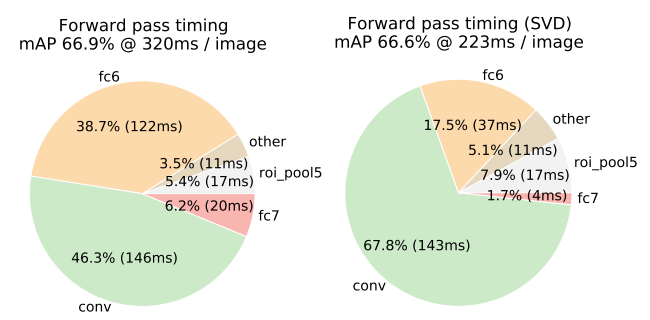
\includegraphics[width=\textwidth]{fig2.png}
    \caption{FCOS的网络架构,其中C3、C4、C5表示骨干网络的特征图,P3到P7是用于最终预测的特征层级。$H \times  W$ 是特征图的高度和宽度。 ‘/s’ ($s = 8,16,\ldots,128$) 是特征图对输入图像层级的下采样率。例子中所有数字都是使用 $800 \times  1024$的输入计算的。}
    \label{fig:fig2}
\end{figure}

遵循 FPN\cite{fpn},我们在不同层级的特征图上检测不同大小的对象。 具体来说,我们使用了五级特征图$P_3,P_4,P_5,P_6,P_7$。 $P_3,P_4,P_5$ 由主干 CNN 的特征图 $C_3,C_4,C_5$ 通过一个$ 1\times 1 $卷积层,以及在\cite{fpn}中自顶向下的连接产生,如图\ref{fig:fig2}所示。$P_6,P_7$分别通过在 $P_5,P_6$上应用一个步幅为2的卷积层产生。 因此,特征级别$P_3,P_4,P_5,P_6$和 $P_7$ 的步长分别为 8、16、32、64 和 128。

与基于锚的检测器将不同大小的锚框分配给不同的特征级别不同,我们直接限制了每个级别的边界框回归的范围。更具体地说,我们首先计算所有特征级别上每个位置的回归目标$ l^\ast, t^\ast, r^\ast$和$ b^\ast$。接下来,如果一个位置满足$\max\left( l^\ast,  t^\ast,  r^\ast,  b^\ast \right) > m_i $或$\max\left( l^\ast,  t^\ast,  r^\ast,  b^\ast \right) < m_{i-1} $,则将其设置为负样本并且因此不再需要回归边界框。这里$ m_i $是特征级别$ i $需要回归的最大距离。在这项工作中,$m_2,m_3,m_4,M_5, m_6$和$m_7$分别设置为0、64、128、256、512和$\infty$。由于具有不同大小的对象被分配到不同的特征级别,并且大多数重叠发生在具有不同大小的对象之间。如果一个位置,即使使用了多级预测,仍然分配给多个地面实况框,我们只需选择面积最小的地面实况框作为其目标。正如我们的实验所示,多级预测可以在很大程度上缓解上述歧义,并将基于 FCN 的检测器提高到与基于锚的检测器相同的水平。

最后,按照\cite{fpn, retinanet},我们在不同特征级别之间共享头部,不仅使检测器参数高效,而且还提高了检测性能。 然而,我们观察到不同的特征级别将回归不同的范围大小(例如,$ P3 $的大小范围为$\left[0,64\right]$和$P4$的范围为$\left[ 64, 128 \right]$),因此为不同的级别使用相同的头部并不合理。因此,我们没有使用标准的$\exp\left(x\right)$,而是使用带有可训练标量$ s_i $的$ \exp\left(s_i x\right) $来自动调整特征级别$ P_i $的指数函数的基数,这略微提高了检测性能。

\subsection{FOCS的center-ness}

在 FCOS 中使用多级预测后,FCOS 和基于锚的检测器之间仍然存在性能差距。 我们观察到这是由于远离对象中心的位置产生了许多低质量的预测边界框。

我们提出了一种简单而有效的策略来抑制这些检测到的低质量边界框,而不会引入任何超参数。 具体来说,我们添加了一个与分类分支并行的\textit{单层分支}(如图\ref{fig:fig2}所示)来预测位置的“center-ness”。center-ness描述了从位置到该位置负责的对象中心的归一化距离,如图 7 所示。给定一个位置的回归目标$ l^\ast, t^\ast, r^\ast$和$ b^\ast$,center-ness目标定义为,
\begin{equation} \label{center-ness}
    \text{centerness}^\ast = \sqrt{\frac{\min\left(l^\ast, r^\ast \right)}{\max\left(l^\ast, r^\ast \right)} \times \frac{\min\left(t^\ast, b^\ast \right)}{\max\left(t^\ast, b^\ast \right)}}
\end{equation}
我们在这里使用\lstinline{sqrt}来减缓中心性的衰减。center-ness的范围是从 0 到 1,因此使用二元交叉熵 (BCE) 损失进行训练。 损失被添加到损失函数方程\ref{equ:total_loss}。测试时,最终分数(用于对检测到的边界框进行排序)是通过将预测的center-ness与相应的分类分数相乘来计算的。因此,center-ness可以降低远离对象中心的边界框的分数。结果,这些低质量的边界框很有可能被最终的非最大抑制(NMS)过程过滤掉,从而显着提高检测性能。

中心度的另一种选择是仅使用真实边界框的中心部分作为正样本,代价是一个额外的超参数,如工作\cite{densebox}所示。 在我们提交之后,[1] 中已经表明,这两种方法的结合可以获得更好的性能。 实验结果见表 3。

\end{document}